\section{Computing a guide path in $C_{reach}$ ($\mathcal{P}_1$) }
\label{rbprm}

We consider the issue of computing a normalized guide path $\mathbf{q}^0(t) : [0,1] \longrightarrow SE(3)$ for the geometrical root of a multiped robot, connecting start and goal configurations. As said in the previous section, the goal is to enforce that any configuration $\mathbf{q}^0$ of the guide is truly feasible, i.e. can be mapped to a configuration in contact. We denote by $C_{contact} \subset SE(3) \times \mathbb{R}^n$ the contact submanifold of the robot.
%~ We say that a root placement $\mathbf{q}^{0}$ is \textit{truly feasible} if there exists $\mathbf{q}^{\overline{0}}$ such that 
%~ $$\mathbf{q}^{0} \oplus \mathbf{q}^{\overline{0}} \in C_{contact} $$
%~ The set of all truly-feasible root placements is denoted by $C_{reach}$. By extension, a trajectory $\mathbf{q}^0(t)$ is truly feasible if $\forall t \in [0,1], \mathbf{q}^0(t) \in C_{reach}$. 
%~ We define a bijective mapping $\pi$ between $C_{reach}$ and $C_{contact}$:
%~ \begin{equation}
    %~ \pi\colon \quad \mathbf{q}^{0} \in C_{reach} \longrightarrow  \mathbf{q}^{0} \oplus \mathbf{q}^{\overline{0}} \in C_{contact} 
    %~ \label{eq:pi}
%~ \end{equation}

We say that a root placement $\mathbf{q}^{0}$ is \textit{truly feasible} if there exists at least one bijective mapping $\pi$
such that
\begin{equation}
    \pi\colon \quad \mathbf{q}^{0} \in  SE(3) \longrightarrow  \mathbf{q}^{0} \oplus \mathbf{q}^{\overline{0}} \in C_{contact} 
    \label{eq:pi}
\end{equation}

The set of all truly feasible root placements is denoted by $C_{reach}$. By extension, a path $\mathbf{q}^0(t)$ is truly feasible if $\forall t \in [0,1], \mathbf{q}^0(t) \in C_{reach}$.

For a two-stage acyclic contact planner to be exact and complete, we need the combination of two conditions on a guide trajectory generator: all the generated trajectories must be \textit{truly feasible} (sufficient condition); the guide planner must be complete, i.e. it must be able to discover any truly feasible trajectory (necessary condition).

In this Section we characterize $C_{reach}$ theoritically with a necessary and a sufficient condition for belonging to the set.
We then describe our implementation of an efficient RRT planner in $C_{reach}$.

   
%~ We want all the configurations of $q^0(t)$ to belong to a set $C_{reach}$ defined as:
%~ 
%~ \begin{eqnarray}
%~ C_{reach}= \{ \mathbf{q}^{0} & : & \exists f, f(\mathbf{q}^{0}) \in C_{contact} \}
%~ \end{eqnarray}
 
\subsection{Conditions for true feasibility}
By default, the true feasibility implies a constructive demonstration by exhibiting a valid $\pi$. This is the approach chosen by \cite{Bouyarmane2009}. However, computing a valid  $\mathbf{q}^{\overline{0}}$ is costly in practice. In this section we rather define a necessary condition and a sufficient condition for true feasibility that do not require this explicit computation.


% and  present the parametrization of a compromise condition used to approximate $C_{reach} \subset SE(3)$, the set of truly feasible configurations. This compromise condition, which we call the reachability condition, is used to compute a relevant guide trajectory using a sampling based motion planner, the Reachability-Based PRM (RB-PRM).


\subsubsection*{True feasibility: necessary condition}
For a contact to be possible, a volume $O_i \in O$ necessarily intersects with the reachable workspace $W(\mathbf{q}^{0})$ (Fig.~\ref{fig:contact_gen}--1). Furthermore, if $\mathbf{q}^{0}$ is truly feasible, then the trunk of the robot $W^0(\mathbf{q}^{0})$ is necessarily not colliding  with the environment $O$.

Therefore we can approximate $C_{reach}$ with a set $C_{reach} \subset C_{reach}^1$ with the reachability condition defined as: 
\begin{equation}
C_{reach}^1 = \{ \mathbf{q}^0 : W(\mathbf{q}^{0}) \cap O \neq \emptyset \wedge W^0(\mathbf{q}^{0}) \cap O = \emptyset \} % \\ }
 %~ & \wedge & A_{trunk}(\mathbf{q}^{root}) \cap W = \emptyset \}
\end{equation}
It is straighforward to prove that  $C_{reach} \subset C_{reach}^1$ (by construction of the included set). 
This inclusion is very important: it directly implies that any motion-planning algorithm with a guaranty of completeness in $SE(3) \times \mathbb{R}^n$ is complete  in $C_{reach} \times \mathbb{R}^n$. This is a strong reduction of the search space, which can be directly applied to any existing method.
 
The condition $C_{reach}^1$ is only necessary which means that one such root placement might not be truly feasible: in practice it is not guaranteed to find a valid sequence of contacts for every guide trajectory in $C_{reach}^1$.

\subsubsection*{Sufficient condition for true feasibility}
%~ In building $C_{reach}^1$, we directly considered the including hull of the root body $W^{0}$, obtaining a necessary condition. 
A trivial sufficient condition for true feasibility can be constructed as a variation of $C_{reach}^1$, by replacing $W^0$ with a bounding volume $B^{max}$ encompassing the whole robot in a given pose, except for the effector surfaces to be in contact (This condition is trivial in the sense that the resulting $W$ has a zero measure. For the need of the proof, the trivial sufficient condition is enough. In practice, the construction of a non-trivial including shape $W^0$ was possible for all the robot structures we considered). We denote by $C_{reach}^\infty \subset C_{reach}$ the set of root placements corresponding to the sufficient condition.

In general, the inclusion is strict, which means that we lose the completeness of the two-stage contact planner (i.e. the planner is not able to discover a trajectory inside $C_{reach} \setminus C_{reach}^\infty$). However, the sufficient condition guarantees that any such trajectories leads to a valid sequence of contacts (i.e. $\pi$ is defined).

\subsection{Reachability: a compromise condition}
The sufficient condition is not  interesting in practice since it leads the solver to lose too many interesting trajectories. The necessary condition is not perfect either, since the first stage of the planner would stop on a guide that is not truly feasible in practice. It might be possible to find a shape $B$ that is necessary and sufficient; however, it seems intuitively very unlikely in general. The construction of a shape $W^0 \subset B \subset B^{max}$ leading to a necessary and sufficient condition (or the proof of its inexistence) is out of the scope of this work.

However between $W^0$ and $B^{max}$, a trade-off can be found between a necessary and a sufficient condition. We define $W^0_s$ as the volume $W^0$ subject to a scaling transformation by a factor $s \in \mathbb{R}^+$. 
%
We then consider the spaces $C_{reach}^s$
 \begin{equation}
C_{reach}^s = \{ \mathbf{q}^0 : W(\mathbf{q}^{0}) \cap O \neq \emptyset \wedge W^0_s(\mathbf{q}^{0}) \cap O = \emptyset \} % \\ }
 %~ & \wedge & A_{trunk}(\mathbf{q}^{root}) \cap W = \emptyset \}
\end{equation}
%
The higher $s$ is, the closer this "reachability condition" is to being sufficient, and if $s=1$, the planner is complete. The parametrization of $s$ allows to find a trade-off between these two desirable properties.
As an example, Figure~\ref{fig:hyq_roms} presents the volumes $W$ computed for the HyQ robot.
In Appendix~\ref{app:rom}, we give a generic method to compute these volumes, with the example of HRP-2.
%~ Section~\ref{sec:results} shows that in practice, it is easy to adjust $s$ to keep most of the interesting guides without introducing incorrect guides.

\begin{figure}
  \centering
  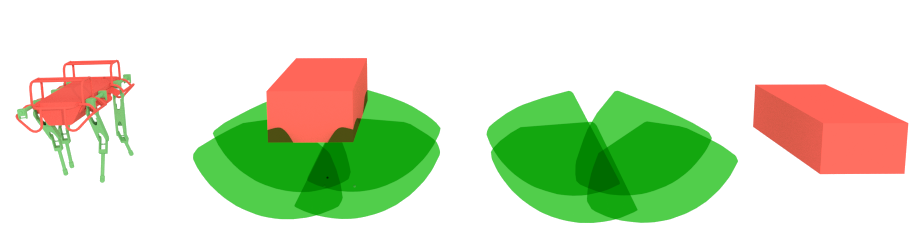
\includegraphics[width=0.95\linewidth]{figures/hyq_roms}
  \caption{
           $W$ volumes for HyQ. The green shapes represent the reachable workspace $W^k$ of each limb. The red shape is $W^0$, a scaling of the convex hull
           of the torso of the robot.}
		   \label{fig:hyq_roms}
\end{figure}

\subsection{Computing the guide trajectory in $C_{reach}^s$}
Once a value of $s$ has been fixed, any sampling-based motion planner can be used to plan a trajectory in $C_{reach}^s$. 
Indeed, contrary to $C_{Contact}$,  $C_{reach}^s$ has a non zero measure in the configuration space $C$. Therefore a standard uniform sampling approach
can work, in spite of a high rejection rate. 
Thus, the only significant change regarding a classical planner is to replace the classical collision checking method with a test of appartenance to $C_{reach}^s$ when verifying
that drawn configurations and associated local paths are valid.

However, to improve the sampling efficiency while remaining probabilistically complete, we bias the sampling process to generate near obstacle configurations, similarly to~\cite{Amato98choosinggood}.
First, a configuration is set to a random point on the surface of one randomly chosen obstacle. The root location is then translated and rotated randomly until the reachability condition is satisfied.
Our current implementation of these modifications is based on the Bi-RRT planner provided by the hpp software.

Thanks to this small set of modifications, the high dimensional truly feasible path planning problem is reduced to a standard geometry and collision checking problem, in a much lower dimension (6 for Hyq, 8 for HRP-2 that has a flexible torso). In so doing we make the problem tractable for sampling based approaches, with extremely efficient computation times.
